% \documentclass[a4paper,titlepage,12pt,twoside,openright,abstracton,headsepline,halfparskip,final,BCOR1.0cm]{scrreprt}
\documentclass[a4paper,titlepage,12pt,twoside,openright,abstracton,headsepline,halfparskip,final,BCOR1.0cm]{scrreprt}
% chapterprefix - erzeugt einen anderen Kopf am Anfang eines Kapitels
% draft - statt final erzeugt leere boxen statt den eingebundenen grafiken
% cleardoublestandard cleardoubleplain cleardoubleempty
% parindent
% footsepline
% halfparskip, halfparskip-, halfparskip* und halfparskip+
% appendixprefix
% liststotoc idxtotoc bibtotoc bibtotocnumbered liststotocnumbered

% Include style for title page, legal clause, and required classes.
% Also sets the page style, header and footer,
% includes severl packages,
% the parameter determines the language of the title logo
\usepackage[german]{cappstyle} % [english]

%% Sprache festlegen
%% Bei einglischer Sprache empfielt sich die Option halfparskip aus der Dokumentenklasse herauszunehmen
\usepackage{ngerman}
%%\usepackage[ngerman]{babel}
% \usepackage[english]{babel}

% Additional packages that anyone can use to her satisfaction
% \usepackage[T1]{fontenc}
% \usepackage{ae,aecompl}
% \usepackage{multirow}
% \usepackage{color}
% \usepackage{floatflt}
% \usepackage{rotating}
% \usepackage{longtable}
% \usepackage{lscape}

%% Change me: Studienarbeit oder Diplomarbeit, Name, Titel
\usepackage[
	bookmarksnumbered=true,
	colorlinks=false,
	pdftitle={Sache},
	pdfsubject={Entwicklung einer Sache},
	pdfauthor={Mein Name},
	pdfcreator={Kile},
	pdfproducer={LaTeX with hyperref package and pdfTeX},
	pdfkeywords={Self-aware Memory, Speicherverwaltung, Speicher, Self-Awareness, Multiprocessor, Management, Memory, intelligent},
	pdfstartpage=1,
	pdfdisplaydoctitle=true,
]{hyperref}
%% Alternatively, use package hyperref with simple settings
% \usepackage[bookmarksnumbered=true,colorlinks=false,pdfdisplaydoctitle=true]{hyperref}

%% Nice cite commands with authors abbreviated into "Karl et al."
% \usepackage[numbers]{natbib}

% Enter your hyphenation list, i.e. hy-phe-na-tion, in order to have these
% words hyphenated correctly at the end of a line. Use spaces to separate 
% words.
\hyphenation{Bin-dung Netz-wer-ma-na-ge-ment}

% Diese Befehle bewirken, dass Absätze  bei Seitenumbrüchen sauberer getrennt
% werden (sog. Schusterjungen und Hurenkinder vermeiden)
\clubpenalty = 10000
\widowpenalty = 10000

%%-------------------------------------------------------------------
%% Weil das Übersetzen mitunter sehr lange dauern kann, lässt sich zum schnelleren
%% Übersetzen mittels \includeonly die Anzahl inkludierter Kapitel reduzieren, 
%% während Dinge wie Seitenzahlen, Inhaltsverzeichnis, Index,etc. erhalten bleiben.
%\includeonly{
% 	Abstract,
% 	Motivation,
% 	Zusammenfassung
%}
%%-------------------------------------------------------------------

\begin{document}

	% make empty pages clear without any header, without any footer
	\pagestyle{empty}

	\capptitle{Studienarbeit}
			{Bachelorarbeit}  % title of thesis
			{Nico Rudolf}                % author name (if desired: cand.-inform.~Name)
			{Prof.~Dr.~rer.~nat.~Wolfgang~Karl}
			{M. Sc. Thomas Becker} % supervisor
			{1. Mai 2018}                               % Anmeldedatum
			{1. September 2018}                                 % Abgabedatum

	\cappclause{Nico Rudolf}          % author name
			{Karlsruhe}    % location
			{01.09.2018}    % date (for legal clause)

	\cleardoublepage
	
%%-------------------------------------------------------------------
	%% Abstract
% 	\begin{abstract}
Diese Arbeit beschäftigt sich..
\end{abstract}


	\begin{abstract}
Diese Arbeit beschäftigt sich..
\end{abstract}


	\cleardoublepage
%%-------------------------------------------------------------------

	\pagestyle{scrheadings}
	\pagenumbering{Roman}

	\pdfbookmark[0]{\contentsname}{Contents} 
	\tableofcontents
	\listoftables
	\listoffigures
% 	\lstlistoflistings
	\cleardoublepage

	\pagestyle{scrheadings}
	\pagenumbering{arabic}
     
%%-------------------------------------------------------------------
	%% Weil das Übersetzen mitunter sehr lange dauern kann, lässt sich mittels
	%% \includeonly oben die Anzahl inkludierter Kapitel reduzieren zum schnelleren
	%% Übersetzen, während Seitenzahlen erhalten bleiben.

	%%-------------------------------------------------------------------

\chapter {Motivation}

Mit der stetig wachsenden Komponentenzahl in modernen Rechensystemen geht eine
Steigerung der Ausfallwahrscheinlichkeit und Fehleranfälligkeit der Komponenten einher.
Eine Möglichkeit die Verlässlichkeit von Rechensystemen zu steigern, ist die Vermeidung von
Fehlern während der Berechnung. Klassische Methoden der Fehlertoleranz wie Checkpoints oder
Redundanz sind allerdings in modernen Systemen aufgrund der Vielzahl der Komponenten
ineffizient und zu teuer. Deshalb ist ein alternativer Ansatz der Verzicht auf die Fehlervermeidung
und auf die Erkennung von Fehlern zu setzen.
Man unterscheidet hierbei zwischen transienten Fehlern (soft errors) und intransienten Fehlern
(hard errors). Soft errors sind von zufälliger und temporärer Natur, das bedeutet, dass ein soft
error während einer Berechnung zu einem fehlerhaftem Ergebnis führen kann, bei Wiederholung
der Berechnung wird dieser Fehler wahrscheinlich jedoch nicht auftreten.
Fehler die dauerhaft existieren, werden als hard errors bezeichnet. Beispiele für hard errors sind
Hardware Ausfälle, denn ein Rechensystem würde unter diesen Umständen dauerhaft falsche
Ergebnisse liefern.
Zurückzuführen sind transiente Fehler auf kosmische Partikel oder elektromagnetische Störfelder.



Diese verursachen unter anderem ungewollte Bitflips in den Registern des Prozessors oder in den Speicherzellen des Hauptspeichers. Das Systeme immer häufiger von transienten Fehlern betroffen sind, ist im wesentlichen auf die niedrigeren Versorgungsspannungen zurückzuführen.
Hintergrund dafür ist der Wunsch nach energieeffizienten Produkten aber auch die zunehmende Integrationsdichte.

Neben der Verfälschung von Berechnungsergebnissen und dem Hervorrufen von kritischen
Systemfehlern, die das System zum Absturz bringen, kann ein transienter Fehler auch folgenlos
bleiben. Um Computersysteme vor solchen Fehlern zu schützen, gibt es mehrere Ansätze, wie die
Redundanz.
Zum Einen gibt es die temporale Rendundanz, bei der eine Berechnung auf dem gleichen System
mehrmals ausgeführt wird. Das berechnete Ergebnis wird dann verglichen und falsche Ergebnisse
werden erkannt. Allerdings bedeutet das, dass die Kosten (Zeit) sich mindestens verdoppeln.
Räumliche Redundanz wird durch die parallele Ausführung auf mehreren (identischen)
Rechensystemen realisiert. Beispielsweise benutzt das Space Shuttle fünf Computersysteme, um
so per Mehrheitsentscheid bestimmen zu können. Die (Hardware-) Kosten steigen hierbei extrem
an, allerdings ist es im Gegensatz zur temporalen Redundanz möglich, nicht nur soft errors
sondern auch hard errors erkannt werden.
Eine Alternative zur teuren Redundanz, stellt eine leichtgewichtige Methode zur Erkennung von
aufgetretenen Fehlern, wie die Symptom-basierte Fehlererkennung, dar.
Die Grundidee ist die Erkennung von Fehlern mittels Abweichungen vom üblichen
Ausführungsverhalten. Das Verhalten wird mittels Metriken, sogenannten Performance Counter,
wie z.B. die Anzahl an TLB Misses, charakterisiert. Zur Festlegung des normalen
Ausführungsverhalten wird eine Datenbank mit Werten verschiedener Ausführungsmetriken von
korrekten Ausführungen angelegt.
Daraufhin werden Ausführungen gezielt mit Fehlern injiziert um die Metriken auf signifikante
Abweichungen zu untersuchen. Zur Laufzeit werden dann die aktuellen Werte mit der Datenbank
verglichen. Sofern die Abweichungen einer oder mehrerer Metriken einen festgesetzten Grenzwert
überschreiten könnte dies als Indikator für diesen Fehler gelten.
Ziel dieser Bachelorarbeit ist die Untersuchung der Anwendbarkeit der Symptombasierten
Fehlererkennung. Dabei wird gezeigt ob das Auftreten von Fehlern oder sogar die aufgetretene
Fehler(-art) bestimmt werden können.

\section{Zielsetzung}

Ziel dieser Bachelorarbeit ist die Untersuchung der Anwendbarkeit der Symptombasierten
Fehlererkennung.
Die Grundidee ist die Erkennung von Fehlern mittels Abweichungen vom üblichen
Ausführungsverhalten. Das Verhalten wird mittels Metriken, sogenannten Performance Counter,
wie z.B. die Anzahl an TLB Misses, charakterisiert. Zur Festlegung des normalen
Ausführungsverhalten wird eine Datenbank mit Werten verschiedener Ausführungsmetriken von
korrekten Ausführungen angelegt.
Daraufhin werden Ausführungen gezielt mit Fehlern injiziert um die Metriken auf signifikante
Abweichungen zu untersuchen. Zur Laufzeit werden dann die aktuellen Werte mit der Datenbank
verglichen. Sofern die Abweichungen einer oder mehrerer Metriken einen festgesetzten Grenzwert
überschreiten könnte dies als Indikator für diesen Fehler gelten.
Dabei wird gezeigt ob das Auftreten von Fehlern oder sogar die aufgetretene
Fehler(-art) bestimmt werden können.


\section{State of the Art}

noch hinzuzufügen , änderung

	\chapter{Material und Methoden}

In diesem Kapitel werden die Materialien und Methoden vorgestellt mit denen die Messungen durchgeführt werden.


\section{Testplattform}
\subsection{HPC Cluster Server}
\subsection{Multicore Computer}
TEST

\section{Metriken als Symptome}

Als Metriken werden in dieser Bachelorarbeit definierte Aktivitäten wie beispielsweise Cache Zugriffe interpretiert. Diese Aktivitäten werden mithilfe von Hardware Perfomance Countern dokumentiert und als Symptome behandelt. Das Perfomance Application Programming Interface (kurz: PAPI) dient dem leichteren Auslesen dieser Perfomance Counter.



\subsection{Hardware Perfomance Counter}

Hardware Perfomance Counter sind spezielle Mehrzweckregister die in modernen Prozessoren
eingebaut sind. Diese Register werden von der on-chip Performance Monitoring Unit (kurz:
PMU) verwaltet und beschrieben.
\cite{PMU}
Das Ziel der PMU ist das Zählen und somit Dokumentieren von Events, wie z.B. Zyklen, Cache Misses oder Floating Point Operations, die im folgenden als Symptome definieren.

Diese Events können in Hardware Events (CPU-Cycles, Instructions, Cache Zugriffe etc,) und Software Events (Page Faults, Context Switche,..) unterschieden werden.

Im Allgemeinen besteht die Hardware zum Zählen der Events aus zwei Komponenten: 

Zum einen die Perfomance Event Select Registers

Diese geben an welche Events überwacht und wie gemessen wird.
Und Event Counters, die als Zielregister für die Werte fungieren.

\begin{figure}[ht]
	\centering
	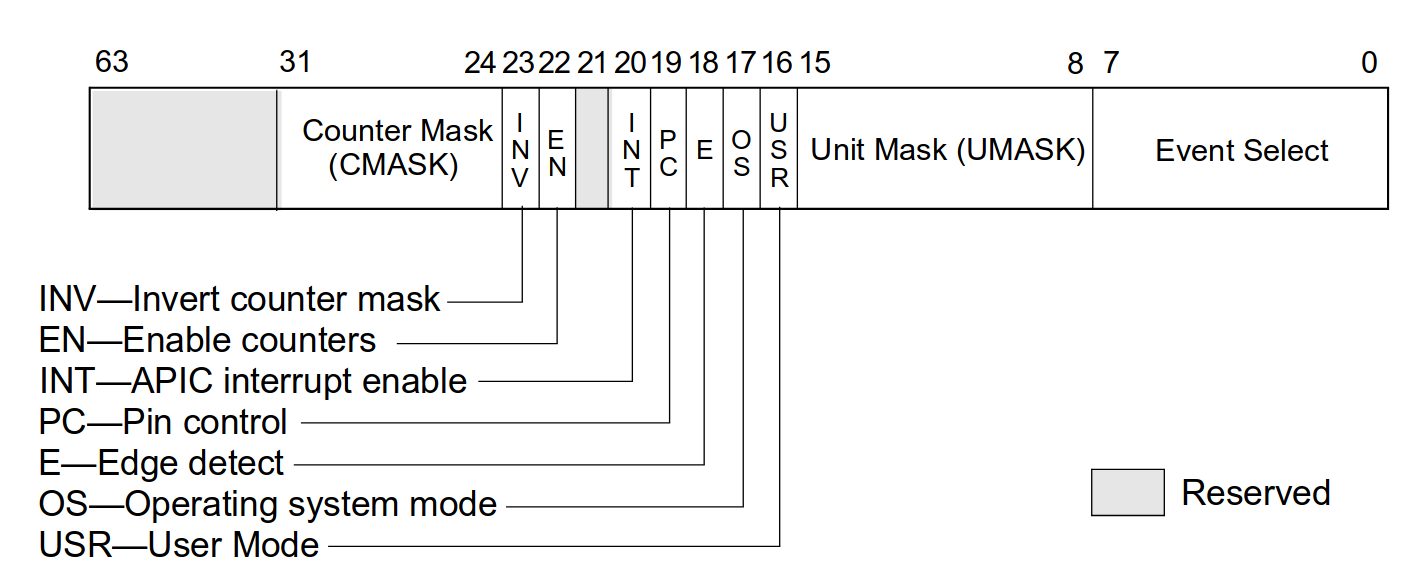
\includegraphics[width=0.8\textwidth]{MSR.png}
	\caption{Intel IA32PERFEVTSELxMSRs (https://software.intel.com/sites/default/files/managed/39/c5/325462-sdm-vol-1-2abcd-3abcd.pdf)}
	\label{fig1}
\end{figure}

Man unterscheidet gemäß Intel zwischen drei Typen von Perfomance Countern:
\begin{itemize} 
	
\item Fixed function counters 
\item General purpose perfomance counters
\item Precise-event based sampling

\end{itemize}

Entwicklung der Perfomance Counter

\begin{figure}[ht]
	\centering
	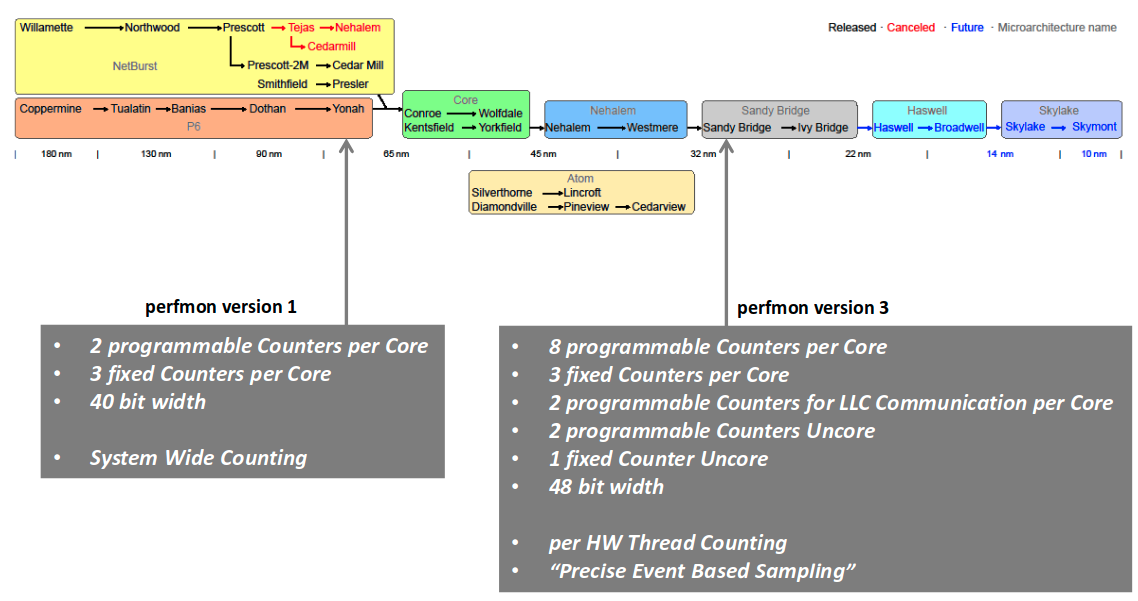
\includegraphics[width=0.8\textwidth]{EvoHPC.png}
	\caption{https://www.inf.ethz.ch/personal/markusp/teaching/263-2300-ETH-spring13/slides/11-perfcounters.pdf}
	\label{fig2}
\end{figure}

Ein Pentium III Prozessor (1999) besitzt zwei Hardware Perfomance Counter, wohingegen ein
aktueller Prozessor wie der Intel Xeon E5-2620 (2014) 634 Perfomance Counter zur Verfügung
stellt, wie der Tabelle im Anhang entnommen werden kann.
\cite{Xeon}

Perfomance Counter werden üblicherweise benutzt um in Abhängigkeit einer Anwendung Hardware auf Engpässe, sogenannte Bottle Necks zu untersuchen. Bottle Necks können typischerweise zu geringer Speicher, geringer Netzwerkdurchsatz oder eine überlastete CPU sein. \cite{HPC} 

Ein Beispiel für die klassische Verwendung ist folgender Programmcode.

\begin{figure}[ht]
	\centering
	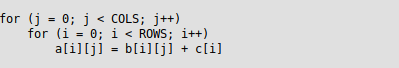
\includegraphics[width=0.8\textwidth]{graphic/Code.png}
	\caption{http://perfsuite.ncsa.illinois.edu/publications/LJ135/x35.html}
	\label{fig3}
\end{figure}

Bei einem unoptimierten Compiler, würden die benachbarten Datenelemente nie nacheinander zugegriffen werden. Messungen an der NCSA Illinois zeigen, dass dies zu einer höheren Anzahl von L2-Cache Misses (212 665 026) führt.


Wenn man allerdings die verschachtelten Schleifen umändert, dass die Matrizen row-by-row basiert durchgegangen werden würde. was der Intel ICC Compiler macht, dann sinken um 11,89 Prozent die L2-Cache Misses auf 25 287 572. Gleichzeitig erfolgt die Berechnung 10-Mal so schnell.
\cite{CacheUnfriendly}


\subsection{Perfomance Application Programming Interface}

Die University of Tennessee entwickelt das Performance Application Programming Interface
(kurz: PAPI) um einen leichteren Zugriff auf perfomance counter anzubieten. Das einheitliche
PAPI-Interface bietet Entwicklern eine Abstraktion der nativen Interfaces und somit eine
vereinfachte Entwicklung. 
PAPI unterstützt alle aktuellen Intel und AMD x86 sowie x8664 Prozessoren (CPU). Durch die
Erweiterung PAPI CUDA wird der Zugriff auf perfomance counter von nVidia Grafikkarten (GPU)
erweitert.
Es wird zwischen high-level interface sowie low-level interface unterschieden. Das high-level
interface bietet einen einfachen sowie schnellen Zugriff, wohingegen das low-level interface
mehr Kontrolle und einen detailliertes Vorgehen erlaubt. In dieser Arbeit wird vor allem das low
level interface benutzt. Informationen über die Implementierungsarbeit ist in Abschnitt 4 zu
finden.
Jede Plattform (CPU, GPU,..) besitzt sogenannte native events, die aus den unterstützen
hardware Performance Countern abgeleitet werden. Die Namen dieser events sind
plattformabhängig. Durch generische preset events abstrahiert PAPI diese nativen events und
ermöglicht dem Entwickler eine einheitliche Sicht ohne exakte Kenntnisse der native events zu
fordern. Sofern ein preset event nicht verfügbar ist versucht PAPI dieses von anderen events
abzuleiten, z.B. Total Number of L2 Cache Misses = L2 Cache Access - L2 Cache Hits.
Die Konfiguration der Events wird durch EventSets ermöglicht. Diese bestehen aus einem oder
mehreren Events und klassifizieren wie die events gemessen werden sollen, z.B. ob der code
im user space oder kernel space ablaufen soll.

\section{Physikalische Fehlerinjektion}

TEST

\subsection{Simulation von defekten CPU-Cores}
TEST

\subsection{Simulation von unzureichender Spannungsversorgung}
TEST
\subsection{Manipulation der Taktfrequenz}
TEST

\subsection{Manipulation der Speicherfrequenz}
TEST

\section{Softwarebasiere Fehlerinjektion}

\subsection{Fehlerinjektion in POSIX Bibliothek}
TEST
\subsection{Fehlerinjektion im Linux Kernel}
TEST

\subsection{Fehlerinjektion zur Laufzeit}
TEST

\section{Benchmarks}
TEST


\subsection{Rodinia Benchmark Suite}
TEST


\subsection{Eigene Benchmarks}
TEST

	\chapter{Messungen}

TEST

\section{Pretests}
TEST
\section{Analyse}
Test
\section{Durchführung der Messungen}
TEST
	\chapter{Evaluation}

TEST

\section{Vergleich der Ausführungsmetriken}
TEST

\section{Indizierung von Fehlerklassen}
TEST

\section{Anwendbarkeit der symptombasierten Fehlererkennung}
TEST


	\chapter{Anwendung der symptombasierten Fehlererkennung}

TEST

\section{Schematische Implementierung}
TEST

\section{Anwendungsfall}
TEST



	\chapter{Zusammenfassung und Ausblick}

TEST


	%\chapter{Symptommetriken}

TEST

\section{Hilfsmittel}
TEST
%	\chapter{Material und Methoden}
Dies ist ein Test


\section{Hammer}

Ziel dieser Bachelorarbeit ist die Untersuchung der Anwendbarkeit der Symptombasierten
Fehlererkennung.
Die Grundidee ist die Erkennung von Fehlern mittels Abweichungen vom üblichen
Ausführungsverhalten. Das Verhalten wird mittels Metriken, sogenannten Performance Counter,
wie z.B. die Anzahl an TLB Misses, charakterisiert. Zur Festlegung des normalen
Ausführungsverha

	% \include{...}

%%-------------------------------------------------------------------
% 	\appendix
% 	\include{...}

%%-------------------------------------------------------------------
	% if all bibtex entries shall be included even without any reference
	%\nocite*{}

	% Suggested style without natbib
	\bibliographystyle{unsrtdin}

	%% Allow nice cite commands from package natbib
%  \bibliographystyle{apalike}
	%% Overview of comamnds available at
	%% http://merkel.zoneo.net/Latex/natbib.php

	% More user styles
	%\bibliographystyle{plain}
	%\bibliographystyle{geralpha}
	%\bibliographystyle{gerplain}
	%\bibliographystyle{itmalpha}
	%\bibliographystyle{itmabbrv}

	\bibliography{Bibliografie}
%%-------------------------------------------------------------------

\end{document}
